\chapter{Análise Bibliográfica sobre Simulação Multiagente e Fenômenos Sociais, por Erick Rodrigues Fraga\label{chap:bibliometria:mutenesss}}

\section{Planejamento do estudo}\label{Virus@mutenesss:questoes}
O planejamento o  desenho do estudo deve descrever as motivações, questões de interesse, escopo, limitações e objetivos do trabalho.

O planejamento do estudo deve motivar o tema escolhido e o interesse do autor.

No caso do meu trabalho, as perguntas que o nortearam foram:
\begin{itemize}
    \item Quais são os temas mais abordados nos artigos?
    \item De que forma a simulação multiagente do tema Virus on Network afeta a nossa vida?
    \item Quais são os principais variáveis independentes e dependentes ligados ao tema Virus on Network?
\end{itemize}

\subsection{O que já existe de pesquisa bibliométrica sobre esse tema?}

Devido a pandemia, houve um aumento muito grande na pesquisa sobre comportamento e transmissão viral. O artigo \cite{maheshwari_network_2020} apresenta o assunto com o foco no COVID=19.

Um exemplo de como a evolução da computação afeta os estudos da transmissão viral pode ser visto no artigo \cite{fain_gpu_2022}

\subsection{Uso do Bibliometrix e Biblioshiny}
Serão usadas a ferramenta e o \textit{workflow} proposto pelos autores do pacote Bibliometrix \cite{aria_bibliometrix_2017}.

\subsection{Limitações}
O exercício relatado foi feito em uma semana, envolvendo entre 8 e 10 horas de trabalho.

\section{Coleta de dados}\label{Virus@mutenesss:coleta}

A coleta de dados feita usando o WoS no dia 28 de novembro de 2022, acessado por meio do Portal de Periódicos da CAPES.

Foi feita uma busca na coleção principal do WoS, visando obter diferentes visualizações sobre o tema, de modo que os resultados esperados viessem tanto da Infectologia quanto da Computação.  


\subsection{Query de Busca}\label{Virus@mutenesss:query}

Foi usada a \textit{query}  de busca ilustrada nas linhas 1 a 6 da listagem \ref{list:query20221128}.

\lstinputlisting[numbers=left, basicstyle=\normalsize\ttfamily,caption=\textit{Query} de busca sobre simulação de transmissão de vírus em um grupo, captionpos=b]{exploratory-data-analysis/mutenesss/Virus/20221128/query.txt} \label{list:query20221128}

\subsubsection{Explicação para os termos de busca usados}\label{Virus@mutenesss:busca}

A busca consistiu de duas cláusulas disjuntivas, unidas por uma conjunção \textit{and}, aplicadas à busca geral.

Os termos \textit{viral}, \textit{virus} e \textit{transmission} (linha 1 da query) foram usados na primeira cláusula da \textit{query}  para recuperar artigos que contenham termos relacionados a transmissão viral em quaisquer formas possíveis.

Os termos \textit{comput*}, \textit{agent}, \textit{multi-agent} e \textit{simulation} (linha 3 da query) foram usados na segunda cláusula da \textit{query} para recuperar artigos que contenham termos relacionados a simulações multi-agentes ou simulações computacionais dos fenômenos de transmissão viral.

O termo \textit{All} (linha 5 da query) representa o escopo da busca, que foi todo o acervo da WoS.

A linha 6 da query representa uma limitação no escopo de resultados da pesquisa, buscando obter apenas os documentos categorizados como Artigos de revista ou Artigos de conferência.

\subsection{Registros recuperados}

Os 1.160 registros obtidos como resultado da busca encontram-se em \url{}. 

Foram utilizadas as opções \textit{Exportar registros para arquivo de texto sem formatação} e \textit{Registro Completo e Referências Citadas} no WoS, para que as citações também fosse usadas em análises da citações (estrutura intelectual do conhecimento). Os 1160 registros foram recuperados em trés blocos de até 500 registros por vez (1-500, 501-1000, 1001-1160).

Informações gerais sobre o dataset Virus@mutenesss estão visíveis na tabela \ref{tab:GeneralInfo:Virus@mutenesss}

\begin{table}[htp]
    \centering
    \csvautotabular[separator=comma]{exploratory-data-analysis/mutenesss/Virus/20221128/Virus@mutenesss_MainInfo.csv}
    \caption{Informações gerais do dataset Virus@mutenesss}
    \label{tab:GeneralInfo:Virus@mutenesss}
\end{table}

\section{Análise dos dados}\label{Virus@mutenesss:analise}

\subsection{Filtragem de registros}
Inicialmente, foram obtidos 1.201 registros, utilizando apenas a query de pesquisa sem quaisquer filtros.

Aplicando um filtro a busca, foram obtidos os 1.160 registros que compõem o \textit{dataset}. Foram mantidos os registros de artigos publicados em revistas científicas e artigos de conferência. Por fim, obtemos o \textit{dataset} que será chamado de Virus@mutenesss.


\subsection{Evolução da Produção Científica}

 \begin{figure}[htp]
     \centering
     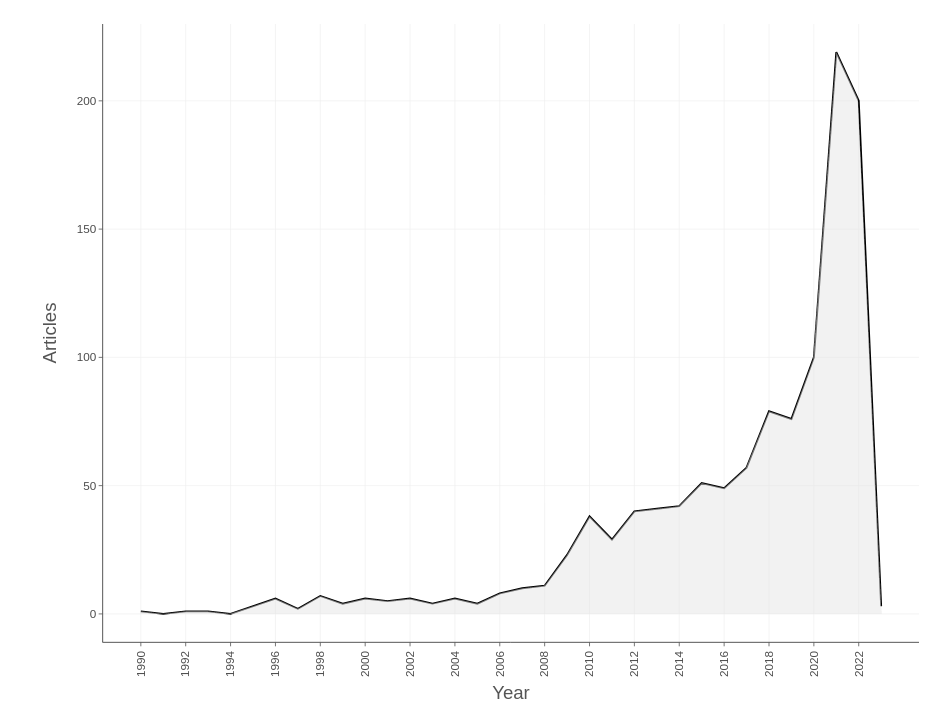
\includegraphics[width=1\textwidth]{exploratory-data-analysis/mutenesss/Virus/20221128/img/AnualProd.png}
     \caption{Evolução da produção científica no \textit{dataset} Virus@mutenesss.}
     \label{fig:evol:anual:Virus@mutenesss}
 \end{figure}

A figura \ref{fig:evol:anual:Virus@mutenesss} apresenta a evolução da produção científica mundial no tema de interesse, segundo o \textit{dataset} Virus@mutenesss. É possível ver um crescimento na produção científica no tema a partir de 2007, com um aumento maior em 2009. Deve ser notado também a explosão em produção em 2018 em seguinte, com assuntos como a COVID-19 e a Influenza cabeceando o aumento.

O \textit{Annual Growth Rate} do \textit{dataset}   é de 3,39\%, sendo bem próximo da taxa média de crescimento da publicação científica mundial, de cerca de 3,3\% anuais, em 2016, como ilustra o estudo em \url{https://www.researchgate.net/publication/333972683_Dynamics_of_scientific_production_in_the_world_in_Europe_and_in_France_2000-2016}, página 23. 

\section{Visualização de Dados}\label{Virus@mutenesss:Data Visualization}

\subsection{Estrutura Conceitual do Conhecimento}

A estrutura conceitual do conhecimento pode ser produzida pela análise de relacionamento estabelecidos entre esses termos. O bibliometrix apresenta um conjunto de técnicas para evidenciar essa estrutura conceitual, e que se organizam em dois grupos:
\begin{description}
     \item [Métricas em rede] que usam grafos para representar relacionamentos entre termos, evidenciando, por meio de métricas de análise de redes sociais, como o conhecimento conceitualmente se organiza.
     \item [Análise Fatorial] Que emprega métricas de redução da dimensionalidade, para explorar, usualmente em mapas bidimensionais, como os termos e palavras se relacionam. 
 \end{description}

 Utilizamos principalmente as métricas em rede para a análise dos dados obtidos com o \textit{dataset} Virus@mutenesss.

 \paragraph{Redes de Co-ocorrências}

 As redes de co-ocorrências apresentam importantes padrões que se formam nas publicações, e podem revelar a estrutura conceitual de uma área do conhecimento.
 A rede foi gerada utilizando o padrão Keywords Plus do Bibliometrix, contendo dois clusters de dados. Cada cluster será analisado separadamente, onde será possível observar um direcionamento presente nas publicações.

\begin{figure}[H]
    \centering
    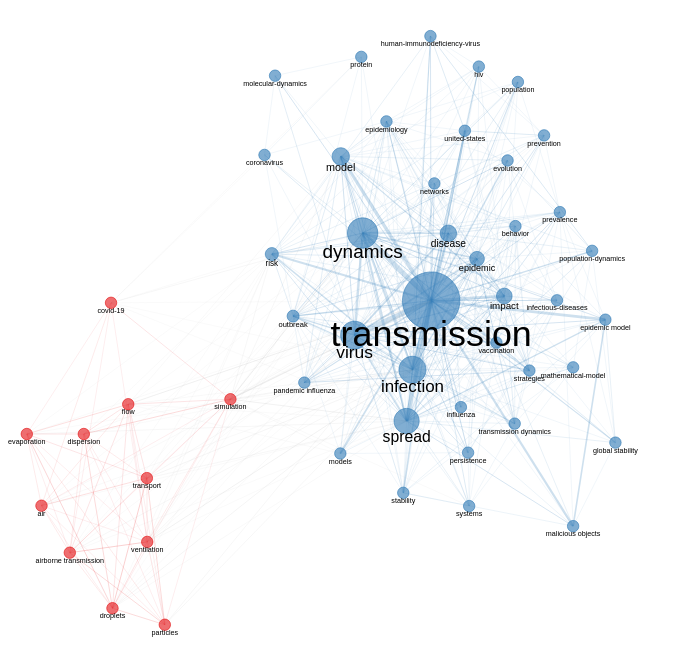
\includegraphics[width=1\textwidth]{exploratory-data-analysis/mutenesss/Virus/20221128/img/Keywordplus_clustering.png}
    \caption{Rede de Co-occorência no \textit{dataset} Virus@mutenesss}
    \label{fig:Coocurrence:Virus@mutenesss}
\end{figure}

 O cluster vermelho na figura \ref{fig:Coocurrence:Virus@mutenesss} demonstra o direcionamento presente em pesquisas recentes no tema, onde podemos visualizar o foco em métodos de transmissão viral de forma aérea.
 Esse foco pode ser percebido com os estudos publicados sobre a COVID-19 e o uso de máscaras afetando a transmissão do vírus.
 
 O cluster azul na figura \ref{fig:Coocurrence:Virus@mutenesss} não indica um direcionamento especificado para a COVID, mas apenas em formas de transmissão viral em geral. É possível ver palavras como \textit{coronavirus}, \textit{influenza}, \textit{epidemic}, \textit{population}, onde todas estão ligadas ao tema central de transmissão viral, representado pelo maior nodo da figura, a palavra \textit{transmission}.

\paragraph{Evolução Temática}
 A evolução temática mostra quais palavras foram mais utilizadas conforme um período de tempo determinado. O gráfico a seguir foi construído dividindo o período de tempo do \textit{dataset} em três partes, e as palavras selecionadas para a montagem foram as Keywords Plus definidas pelos autores.

 \begin{figure}[h]
     \centering
     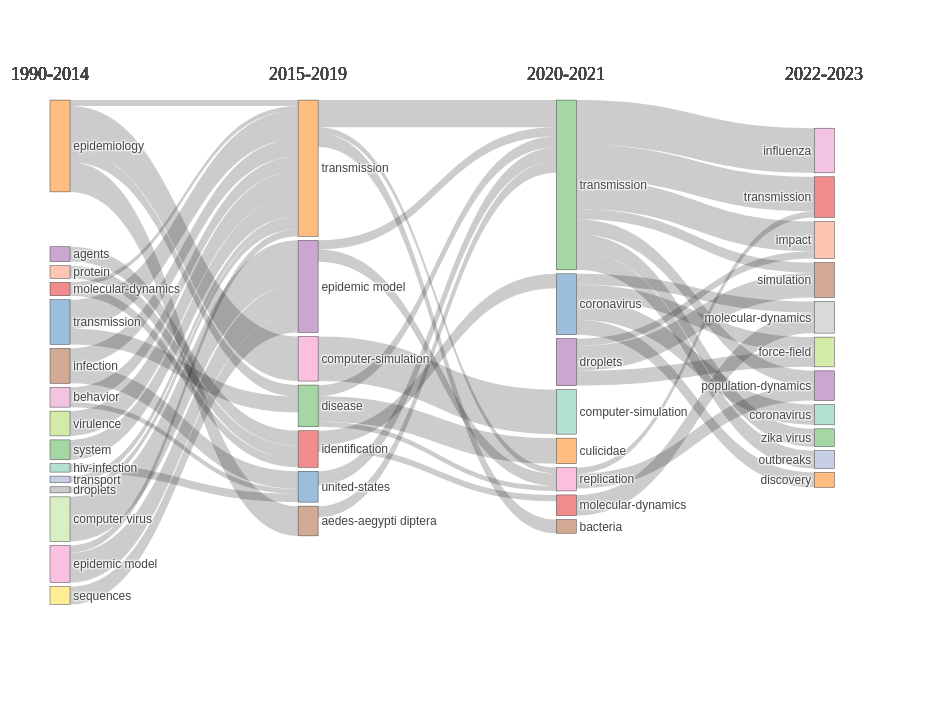
\includegraphics[width=1\textwidth]{exploratory-data-analysis/mutenesss/Virus/20221128/img/thematic_evo.png}
     \caption{Evolução temática do \textit{dataset} Virus@mutenesss}
     \label{fig:Thematic_Evo:Virus@mutenesss}
\end{figure}

Um ponto importante a ser observado é a permanência da palavra \textit{transmission} durante todos os períodos observados, e o crescimento das palavras \textit{computer simulation} ou \textit{simulation} a partir de 2015, demonstrando um crescimento na importância da simulação desses fenômenos, visando os entender melhor.

\subsection{Estrutura Intelectual do Conhecimento}

Conhecimento científico é produzido por processos intelectuais onde autores de trabalho escolhem deliberadamente referenciar trabalhos de outros, por meio de documentos publicados, que são encaminhados para publicações em fontes de informação de sua escolha, e que evoluem ao longo do tempo.

 O Bibliometrix permite exploração da estrutura intelectual do conhecimento, usando basicamente duas abordagens:
 \begin{itemize}
     \item Redes de Co-Citação, abordagem bastante comum;
     \item Historiografia, abordagem pouco usual.
\end{itemize}
Utilizaremos aqui apenas as Redes de Co-Citação para análise de dados.

\subsubsection{Redes de Co-Citação}

\begin{figure}[H]
     \centering
     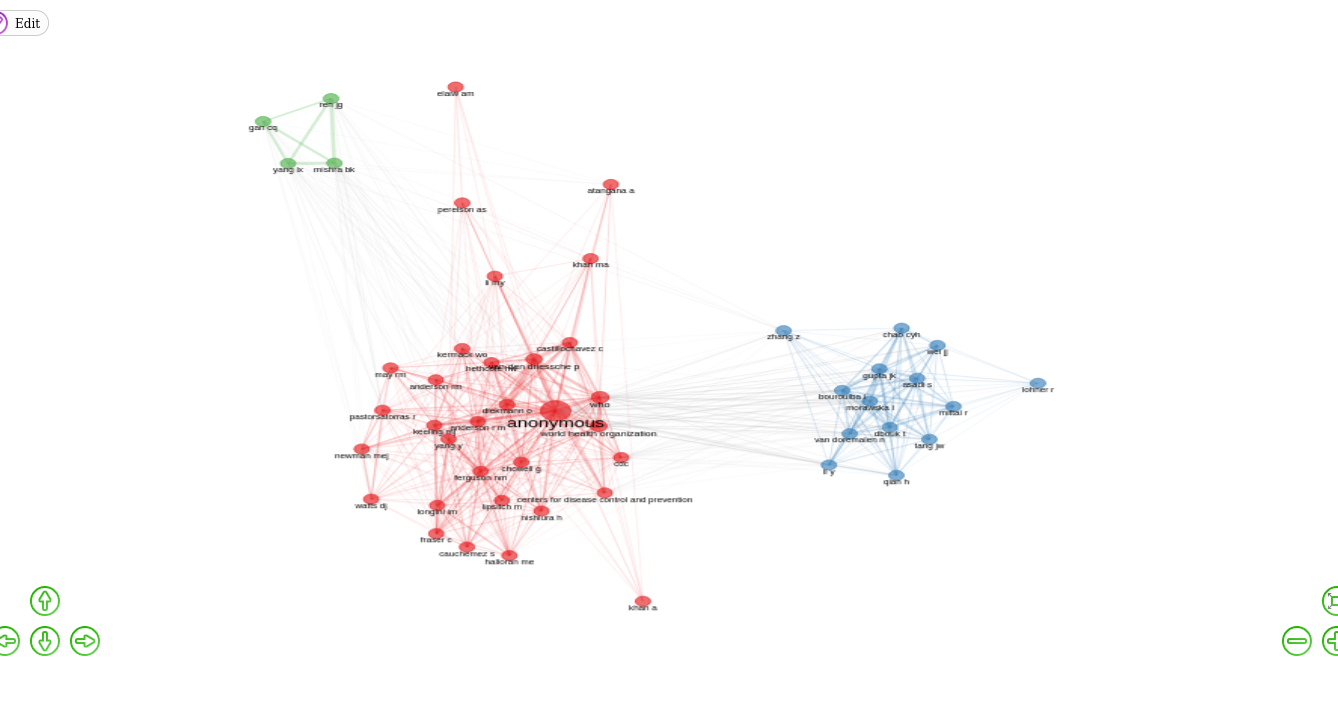
\includegraphics[width=1\textwidth]{exploratory-data-analysis/mutenesss/Virus/20221128/img/CocitationNetwork.png}
     \caption{Rede de cocitação entre as 50 referências mais presentes no  \textit{dataset} Virus@mutenesss.}
     \label{fig:Cocit:Virus@mutenesss}
\end{figure}

Analisando a imagem, é possível perceber três principais grupos de citação entre si. Ainda assim, todos tem um retorno para o grupo vermelho, com muitas citações retornando ao \textit{CDC} ou \textit{Centers for Disease Control and Prevention}, \textit{WHO} ou \textit{World Health Organization} e para \textit{Anonymous}.


\subsection{Estrutura Social  do Conhecimento}

\subsubsection{Mapa de Colaboração Mundial}

Observando a imagem \ref{fig:Comap:Virus@mutenesss} podemos perceber que o tema é algo pesquisado em todo o mundo. A seguir, iremos observar tabelas com as quantidades de colaborações dos países, com o foco nos países com no mínimo 5 colaborações entre eles.

\begin{figure}[h]
      \centering
      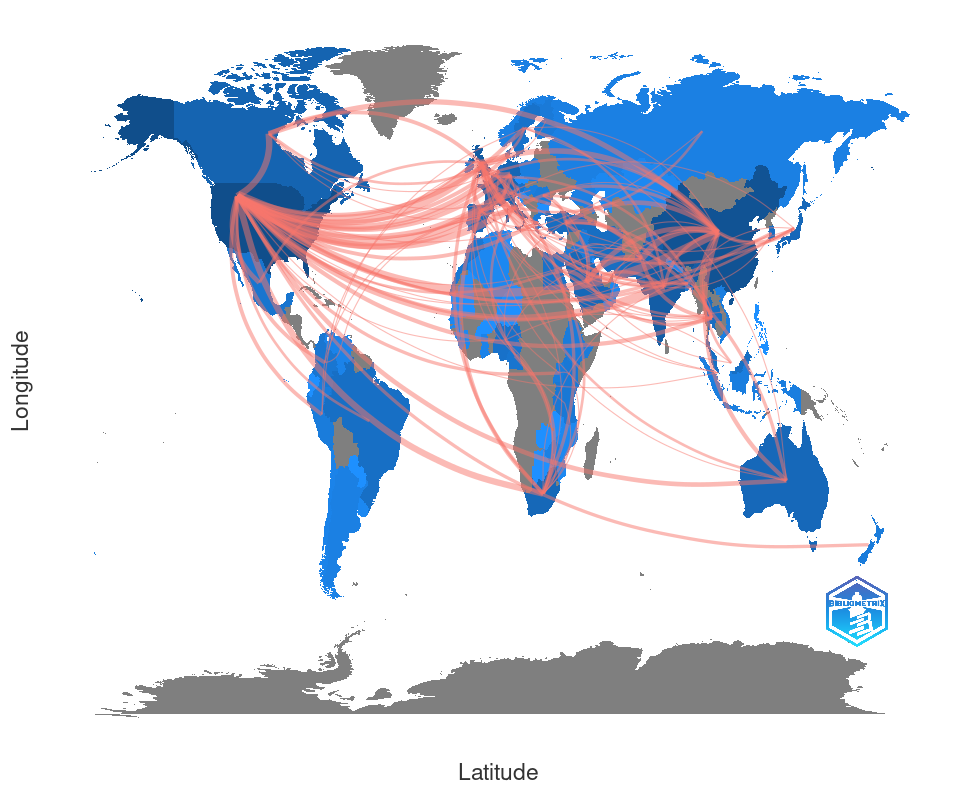
\includegraphics[width=1\textwidth]{exploratory-data-analysis/mutenesss/Virus/20221128/img/worldcolab.png}
      \caption{Mapa de Colaboração Mundial no \textit{dataset} Virus@mutenesss}
      \label{fig:Comap:Virus@mutenesss}
  \end{figure}
\subsection{Tabela de Colaboração Mundial}

\begin{table}[htp]
    \centering
\begin{tabular}{|l|l|l|}
\hline
From           & To             & Frequency \\ \hline
CHINA          & JAPAN          & 5         \\
FRANCE         & ITALY          & 5         \\
FRANCE         & SOUTH AFRICA   & 5         \\
PAKISTAN       & THAILAND       & 5         \\
SAUDI ARABIA   & TURKEY         & 5         \\
UNITED KINGDOM & CANADA         & 5         \\
UNITED KINGDOM & INDIA          & 5         \\
USA            & COLOMBIA       & 5         \\
USA            & DENMARK        & 5         \\
USA            & GREECE         & 5         \\
USA            & PERU           & 5         \\
CHINA          & AUSTRALIA      & 6         \\
SAUDI ARABIA   & EGYPT          & 6         \\
UNITED KINGDOM & FRANCE         & 6         \\
USA            & BELGIUM        & 6         \\
USA            & GERMANY        & 6         \\
USA            & SWEDEN         & 6         \\
USA            & THAILAND       & 6         \\
CHINA          & TURKEY         & 7         \\
SOUTH AFRICA   & CAMEROON       & 7         \\
UNITED KINGDOM & ITALY          & 7         \\
USA            & AUSTRALIA      & 7         \\
USA            & MEXICO         & 7         \\
CHINA          & SAUDI ARABIA   & 8         \\
PAKISTAN       & TURKEY         & 8         \\
USA            & NETHERLANDS    & 8         \\
USA            & SPAIN          & 8         \\
CHINA          & CANADA         & 9         \\
CHINA          & UNITED KINGDOM & 10        \\
USA            & SWITZERLAND    & 10        \\
PAKISTAN       & SAUDI ARABIA   & 11        \\
UNITED KINGDOM & GERMANY        & 11        \\
USA            & CANADA         & 13        \\
USA            & SOUTH AFRICA   & 13        \\
CHINA          & PAKISTAN       & 14        \\
USA            & INDIA          & 15        \\
USA            & ITALY          & 15        \\
USA            & FRANCE         & 18        \\
USA            & CHINA          & 23        \\
USA            & UNITED KINGDOM & 42        \\ \hline
\end{tabular}
\end{table}\label{tab:WorldColab:Virus@mutenesss}

A tabela \ref{tab:WorldColab:Virus@mutenesss} representa a frequência de pesquisa realizada entre países. A tabela foi limitada para que os países presentes houvessem no mínimo 5 colaborações.

Observaremos também as tabelas de colaboração da China e dos EUA, que são os dois países líderes em pesquisas no tema, conforme apresentado no \textit{dataset}.

\subsection{Tabela de Colaboração Mundial - China}

\begin{longtable}{@{}|l|l|l|@{}}
\toprule
From  & To              & Frequency \\* \midrule
\endfirsthead
%
\endhead
%
\bottomrule
\endfoot
%
\endlastfoot
%
CHINA & AUSTRALIA       & 6         \\
CHINA & AUSTRIA         & 1         \\
CHINA & BELGIUM         & 1         \\
CHINA & CANADA          & 9         \\
CHINA & COLOMBIA        & 1         \\
CHINA & ECUADOR         & 1         \\
CHINA & FRANCE          & 1         \\
CHINA & GERMANY         & 1         \\
CHINA & GHANA           & 1         \\
CHINA & INDIA           & 4         \\
CHINA & INDONESIA       & 1         \\
CHINA & IRAN            & 2         \\
CHINA & IRELAND         & 1         \\
CHINA & ITALY           & 4         \\
CHINA & JAPAN           & 5         \\
CHINA & JORDAN          & 1         \\
CHINA & KAZAKHSTAN      & 1         \\
CHINA & KOREA           & 2         \\
CHINA & KUWAIT          & 1         \\
CHINA & LUXEMBOURG      & 1         \\
CHINA & MALAYSIA        & 3         \\
CHINA & MOROCCO         & 1         \\
CHINA & NETHERLANDS     & 3         \\
CHINA & NEW ZEALAND     & 1         \\
CHINA & NIGERIA         & 1         \\
CHINA & OMAN            & 1         \\
CHINA & PAKISTAN        & 14        \\
CHINA & PERU            & 1         \\
CHINA & PHILIPPINES     & 1         \\
CHINA & ROMANIA         & 2         \\
CHINA & RUSSIA          & 1         \\
CHINA & SAUDI ARABIA    & 8         \\
CHINA & SINGAPORE       & 1         \\
CHINA & SOUTH AFRICA    & 1         \\
CHINA & SPAIN           & 1         \\
CHINA & SWEDEN          & 2         \\
CHINA & TANZANIA        & 1         \\
CHINA & THAILAND        & 4         \\
CHINA & TURKEY          & 7         \\
CHINA & U ARAB EMIRATES & 2         \\
CHINA & UNITED KINGDOM  & 10        \\* \bottomrule
\caption{Colaborações Mundiais da China no \textit{dataset} Virus@mutenesss}
\label{tab:ChinaWorldColab:Virus@mutenesss}
\end{longtable}


\subsection{Tabela de Colaboração Mundial - EUA}

% Please add the following required packages to your document preamble:
% \usepackage{longtable}
% Note: It may be necessary to compile the document several times to get a multi-page table to line up properly
\begin{longtable}{|l|l|l|}
\hline
From & To             & Frequency \\ \hline
\endfirsthead
%
\endhead
%
\hline
\endfoot
%
\endlastfoot
%
USA  & AUSTRALIA      & 7         \\
USA  & AUSTRIA        & 3         \\
USA  & BANGLADESH     & 3         \\
USA  & BELGIUM        & 6         \\
USA  & BOTSWANA       & 1         \\
USA  & BRAZIL         & 3         \\
USA  & BURKINA FASO   & 1         \\
USA  & CANADA         & 13        \\
USA  & CHINA          & 23        \\
USA  & COLOMBIA       & 5         \\
USA  & CYPRUS         & 1         \\
USA  & DENMARK        & 5         \\
USA  & ECUADOR        & 1         \\
USA  & EGYPT          & 3         \\
USA  & FRANCE         & 18        \\
USA  & GERMANY        & 6         \\
USA  & GREECE         & 5         \\
USA  & INDIA          & 15        \\
USA  & IRAN           & 2         \\
USA  & IRELAND        & 2         \\
USA  & ISRAEL         & 1         \\
USA  & ITALY          & 15        \\
USA  & JAPAN          & 3         \\
USA  & JORDAN         & 1         \\
USA  & KENYA          & 1         \\
USA  & KOREA          & 4         \\
USA  & MALAWI         & 1         \\
USA  & MALAYSIA       & 1         \\
USA  & MAURITANIA     & 1         \\
USA  & MEXICO         & 7         \\
USA  & NEPAL          & 2         \\
USA  & NETHERLANDS    & 8         \\
USA  & NEW ZEALAND    & 4         \\
USA  & NIGERIA        & 2         \\
USA  & PAKISTAN       & 1         \\
USA  & PERU           & 5         \\
USA  & PORTUGAL       & 1         \\
USA  & RUSSIA         & 2         \\
USA  & SAUDI ARABIA   & 2         \\
USA  & SENEGAL        & 1         \\
USA  & SIERRA LEONE   & 1         \\
USA  & SINGAPORE      & 2         \\
USA  & SOUTH AFRICA   & 13        \\
USA  & SPAIN          & 8         \\
USA  & SWEDEN         & 6         \\
USA  & SWITZERLAND    & 10        \\
USA  & TANZANIA       & 1         \\
USA  & THAILAND       & 6         \\
USA  & TURKEY         & 1         \\
USA  & UGANDA         & 4         \\
USA  & UNITED KINGDOM & 42        \\
USA  & VENEZUELA      & 1         \\
USA  & ZAMBIA         & 1         \\ \hline
    \caption{Colaborações Mundiais do EUA no \textit{dataset} Virus@mutenesss}
    \label{tab:USAWorldColab:Virus@mutenesss}
\end{longtable}

\section{Conclusões}

O tema \textit{Virus on Network} é um tema que recebeu muita atenção em anos recentes devido ao surgimento da COVID-19, trazendo assim uma nova visualização sobre como vírus em geral são transmitidos em grupos sociais.

O estudo dessa área é algo que pode ser visto de forma global, seja em seres humanos ou animais, tornando assim mais importante o entendimento desse tema.

Exemplos de estudos dessa área podem ser vistos nos seguintes artigos:
\begin{itemize}
    \item \cite{manout_assessing_2021} - Mostra os efeitos que o meio que vivemos afeta a transmissão viral, utilizando o COVID-19 como exemplo.
    \item \cite{noauthor_complex_nodate} - Mostra a importância do meio na transmissão viral, utilizando o compartilhamento de seringas como meio.
    \item \cite{dion_landscape_2011} - Fala sobre os métodos de transmissão da Foot-and-Mouth disease em búfalos e gado na África.
    \item \cite{fain_gpu_2022} - Mostra o efeito do progresso computacional para a simulação multiagente, reduzindo o tempo necessário para estudar os fenômenos virais.
    \item \cite{ferguson_epidemiological_2018} - Apresenta um modelo epidemiológico baseado em registros anteriores, focado na IHNV, que afeta peixes.
\end{itemize}


Embora o trabalho esteja incompleto, ele apresenta o arcabouço geral de informações que possibilitam responder parcialmente às  questões formuladas no início da pesquisa, em \ref{Virus@mutenesss:questoes}, para a qual serão apresentadas breves respostas preliminares:

\begin{itemize}
    \item Quais são os temas mais abordados nos artigos?
    \subitem Os principais temas é a transmissibilidade de vírus entre grupos. Exemplos desses vírus estudados em seres humanos são a COVID-19, a Influenza e o HIV. Exemplos desses vírus em animais são o IHNV(infectious hematopoletic necrosis virus), que foi observado em um conjunto de peixes, e o Foot-and-Mouth Disease, que foi observado em Búfalos e Gado na África.
    \item De que forma a simulação multiagente do tema Virus on Network afeta a nossa vida?
    \subitem Estudar como o vírus trafega nas redes nos permite encontrar formas que diminuam o impacto deles na sociedade, diminuindo assim o seu risco para a sociedade. Exemplos dessas formas são o uso de máscaras e a vacinação, como pode ser visto com a COVID-19.
    \item Quais são os principais variáveis independentes e dependentes ligados ao tema Virus on Network?
    \subitem Como variáveis independentes, podemos ver coisas como a transmissibilidade do vírus, a chance de ir testar se está contaminado, a chance de obter resistência a um vírus, a mortalidade e a chance de recuperação.
    Como variáveis dependentes, podemos observar a quantidade de agentes e o local onde os agentes estão envolvidos.
\end{itemize}
